\begin{figure}
    \centering
        \begin{subfigure}{.5\textwidth}
        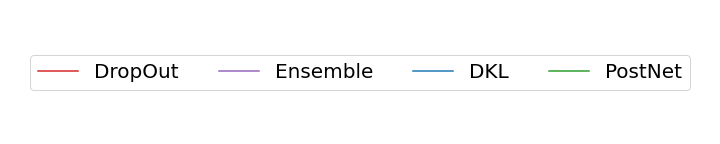
\includegraphics[width=\textwidth]{sections/011_icml2022/resources/legend.png}
    \end{subfigure}
    \vspace{-5mm}
    
    \begin{subfigure}{.4\textwidth}
        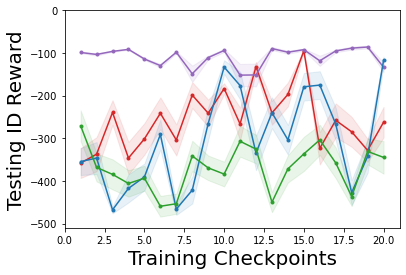
\includegraphics[width=\textwidth]{sections/011_icml2022/resources/Acrobot-v1-mean_reward_-testing-model.png}  
    \end{subfigure}
    \begin{subfigure}{.4\textwidth}
        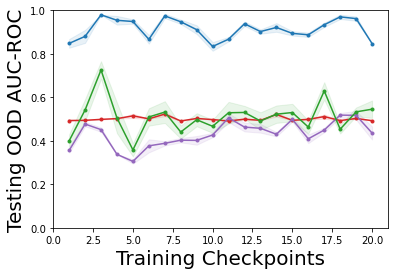
\includegraphics[width=\textwidth]{sections/011_icml2022/resources/AcrobotOOD-v0-AUC-ROC-epistemic_-testing-model.png}
    \end{subfigure}
    \caption{Comparison of the testing performance of the four uncertainty methods using epsilon-greedy strategies at training and testing time on Acrobot. Ideally, an uncertainty aware-model should achieve high reward and high OOD detection scores.}
    \label{fig:model-testing-performance-acrobot}
\end{figure}